% This is a template to create your midterm report as a pdf.
% Just fill in the areas and run pdflatex
% For more information on LaTeX documents consult The (Not So
% Short Introduction to LateX2e
%
% to compile your report use the command
% pdflatex reportdocument.tex
%
% if you have \ref useage or other cross links
% you will have to run the above command again

% set 12pt font
\documentclass[12pt]{article}
% some useful packages
\usepackage[pdftex]{graphicx,color}
\usepackage{lscape}
\usepackage{hyperref}
\usepackage{fullpage}
\def\baselinestretch{1.5} % line spaceing
% set title
\title{Midterm Report \\
ECE437: Computer Architecture}
% fill in the blanks
\author{Jevin Sweval \\
        TA: Abhisek Pan}
% \today will put todays date
% or you can manually put the date in
\date{2010-03-05}
% cover page is a page by itself

\begin{document}
  \maketitle
  \newpage

% executive overview remember
% this should be on a page by itself
\section{Executive Overview}
As part of the ECE437 course, I have realized a MIPS-subset CPU in single-cycle and pipelined form that is synthesizable for the Cyclone II FPGAs. The subset of MIPS implemented allows for general purpose computing while still keeping the design simple. The first design completed, the single-cycle implementation, introduced me to the major components of the CPU: memory, ALU, control logic, and the register file. The register file and ALU were implemented by myself while the RAM was provided by the course. After verification of their correctness, the rest of the single-cycle CPU was built around them. This implementation was important in teaching me how to better debug complex designs with many signals --- a skill that proved to be crucial to my pipelined design. The single-cycle CPU works correctly for all test cases, runs at 22~MHz, and has an average CPI of $\approx 1.2$.\\

The pipelined implementation was built upon the single-cycle implementation. It broke up the CPU into the classic RISC pipeline: IF, ID, EX, MEM, and WB stages. This implementation gave me insight into the problems with the complex hazards in a pipelined processor. Multiple in-flight instructions and a plethora of signals made this design even more difficult to debug. By forsaking a data forwarding unit, the design was simplified and correct functionality was achieved. This design passes all tests, runs at 75~MHz, and has an average CPI of $\approx 2.5$. In the rest of this report I will detail the design of the CPUs, do debugging exercises, and discuss the results obtained from the designs.\\

\newpage
\section{Processor Design}

Both the single-cycle and pipelined designs that I implemented closely followed the course textbook's designs. I feel that the most significant design choice was my coding methodology. Both designs are coded almost entirely in behavioral VHDL. I find this type of code to be much easier to write and debug because it can be single-stepped in a debugger yet, if written carefully, can compile down to logic that is just as efficient as a structural design. Also central to my coding methodology were VHDL records. The input and output signals to a block were wrapped in a record (similar to C \texttt{struct}s). Using records, one can add and remove signals to blocks without the time-consuming and error-prone edits of port and entity declarations. The records also group the signals in the waveform viewer, allowing for a tidier waveform window. I extensively use \texttt{numeric\_std} types and operators in my code to vastly cut down on code size (my ALU was two lines of code per operation) and to let the synthesizer automatically schose the best implementation in hardware. Most non-numeric types are declared as enumeration types. For example, the instructions are decoded into opcode enumerations. These enumerated types are human-readable in waveforms and source code instead of appearing as indecipherable bitstrings.\\

My single-cycle design was quite straightforward and consisted mainly of the register file, ALU, instruction/data memories, and control logic. The CPI of this design is very close to 1 because every single instruction takes just 1 cycle except for \texttt{lw} and \texttt{sw} instructions which take 2 cycles due to 2-cycle memory access. The long critical paths prevent the design from running at high clock speeds. The pipelined design reuses most parts of the single-cycle design while adding a memory arbiter (to control access to the now shared memory), pipeline registers, and hazard detection. Because the logic elements of the FPGA each have a DFF, the additional pipeline registers did not occur much overhead. Most of the registers were merged into already existent logic elements. In this aspect, the pipelining was ``free''. Due to time constraints I did not implement any forwarding logic, meaning that any dependent instructions will stall the pipeline. Despite this, the CPI of the pipelined design was not terrible, as discussed in the Results section. Also discussed in that section is how the RAM is the bottleneck of the design. This means that it might be possible to add forwarding logic (decreasing CPI) without lowering f$_{\textrm{max}}$.

\newpage

\begin{landscape}

\begin{figure}
	\begin{center}
		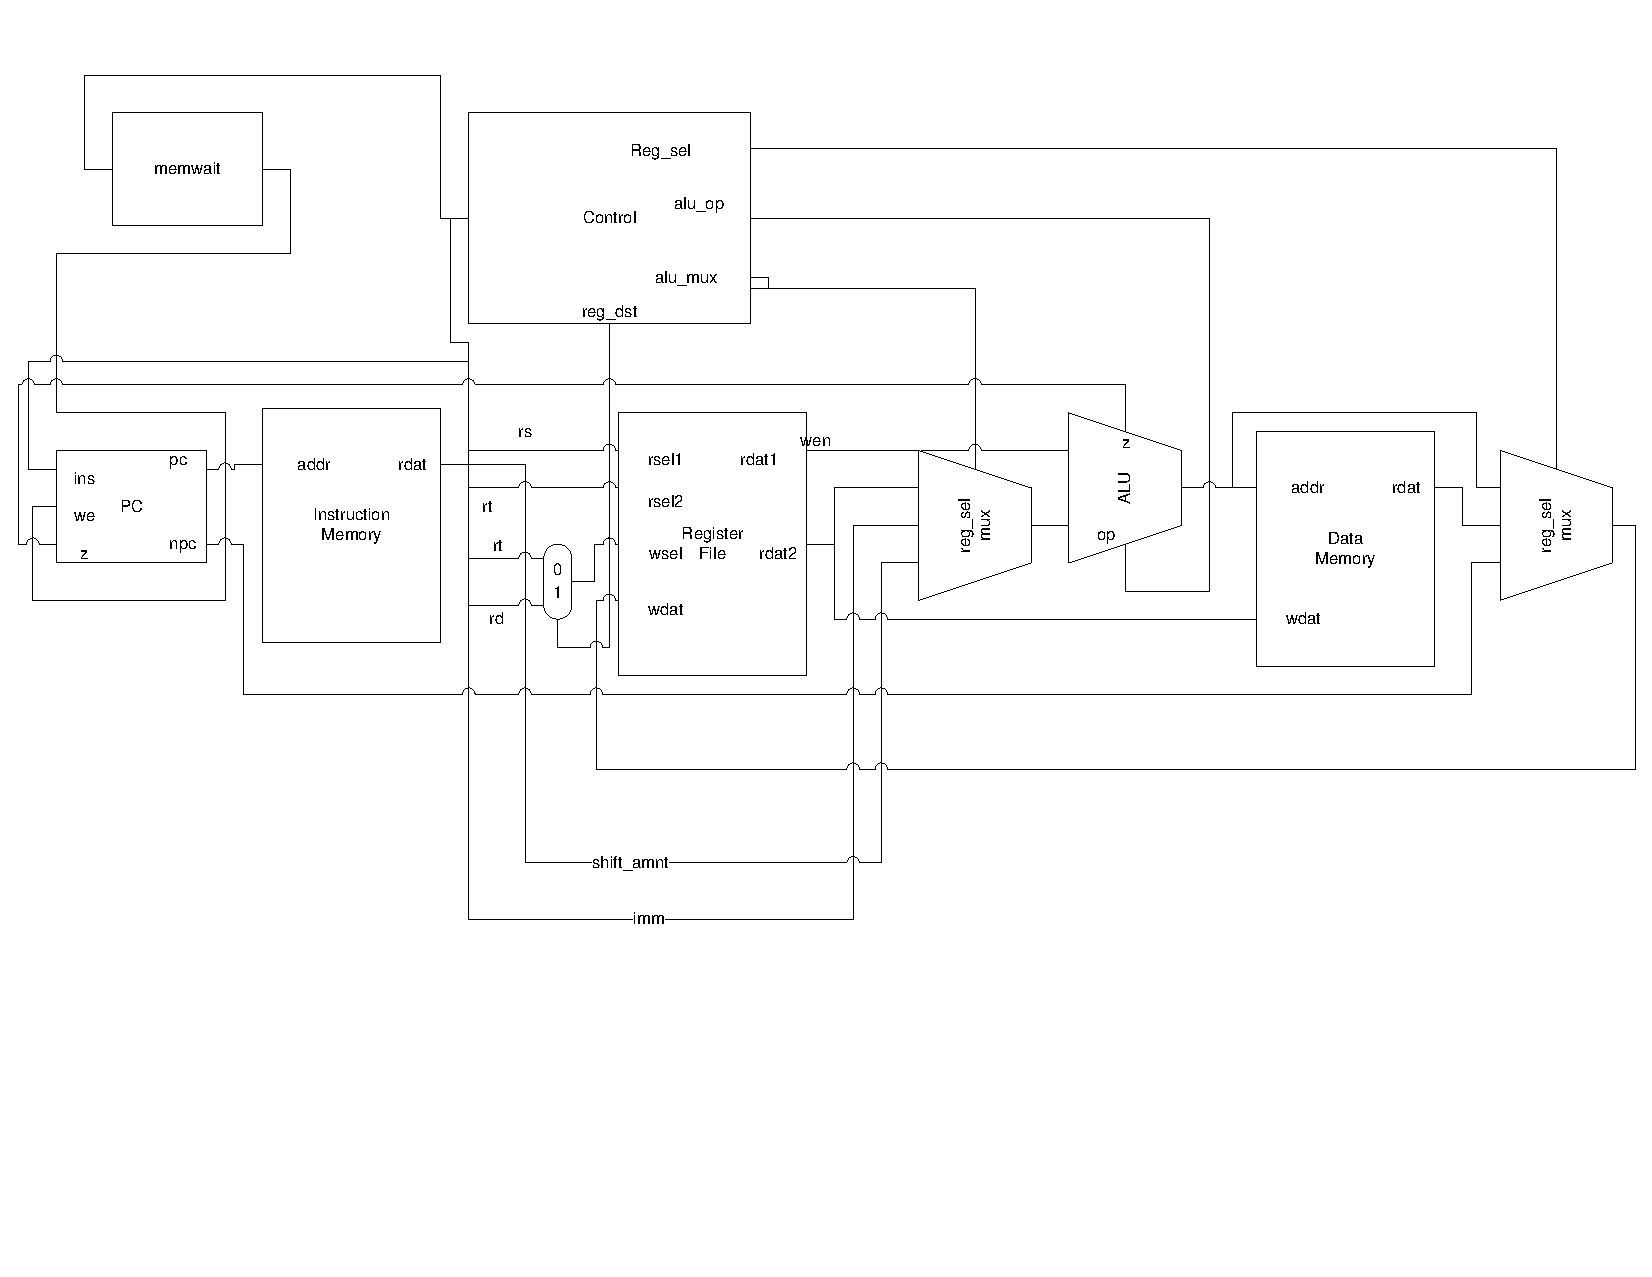
\includegraphics[width=7in]{bld}
	\end{center}
	\caption{Single-cycle Block Diagram}
	\label{fig:scbld}
\end{figure}

\end{landscape}

\newpage

\begin{landscape}

\begin{figure}
	\begin{center}
		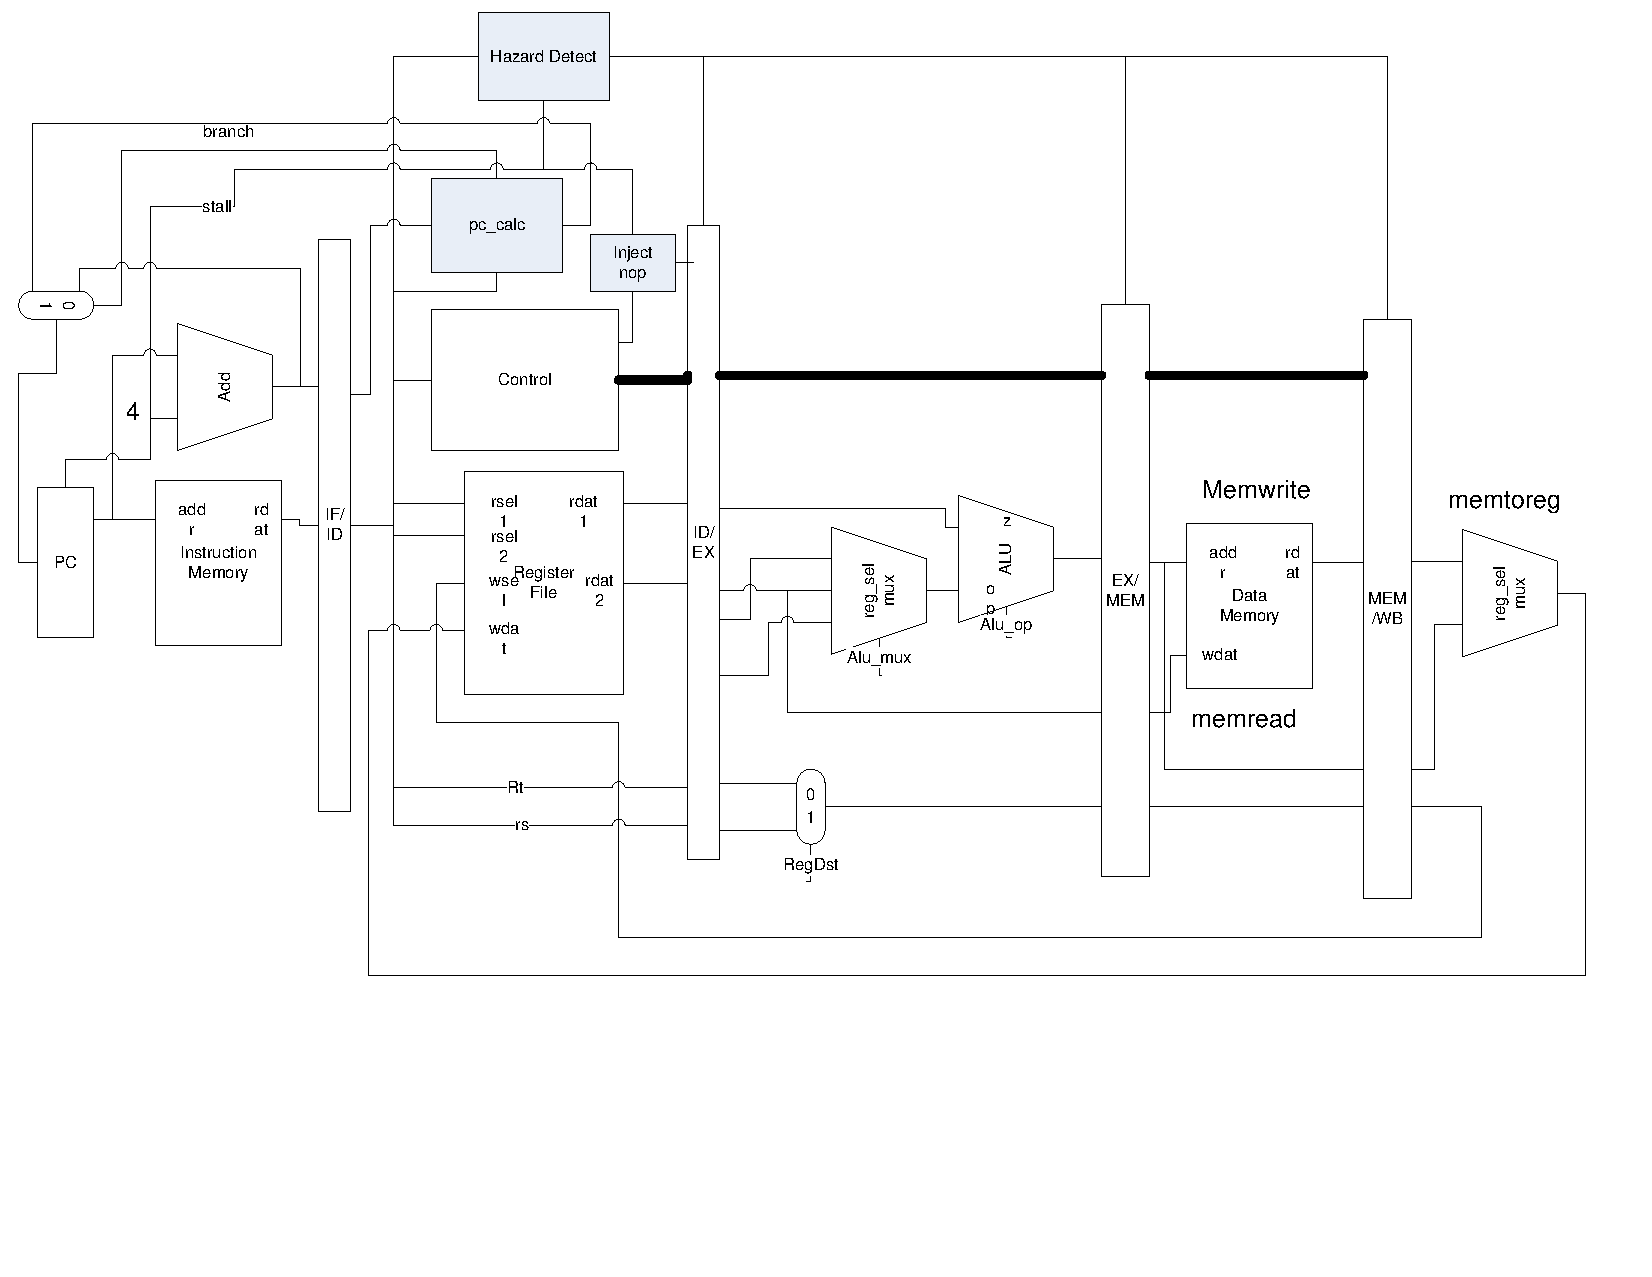
\includegraphics[width=7in]{bld_pipeline_branch}
	\end{center}
	\caption{Single-cycle Block Diagram}
	\label{fig:scbld}
\end{figure}

\end{landscape}

\newpage

\newpage
\section{Processor Debug}

The output of the CPU is incorrect  because the \texttt{sw} instruction never actually wrote the value to memory.  The value \texttt{0x0000BEEF} should have been written to address \texttt{0x00000100}. One possible explanation for this behavior is a bug in the ID control logic. If the \texttt{sw} instruction was decoded incorrectly such that the \texttt{mem\_write} signal was not asserted, the instruction will never write to memory. The \texttt{mem\_write} signal originates from the control block in the ID stage and simply propagates through the pipeline registers until it reaches the MEM stage where it is consumed by the memory block. To find this bug, I would look at the \texttt{mem\_write} signal to ensure it is generated correctly by the control block and propigated by the pipeline registers correctly to the memory block.\\

Another possible explanation is that the controller which arbitrates access to the shared memory block is incorrect. If this is the case, even with a correct \texttt{mem\_write} signal, it is possible that the processor tries to perform a memory write operation while the \texttt{vram} block is not in the \texttt{ready} or \texttt{idle} state, resulting in no write. In this case, the problem originates at the memory arbiter and propagates when the arbiter fails to stall the pipeline until a \texttt{ready} or \texttt{idle} state. I could detect this by checking to make sure that \texttt{mem\_write} is only asserted when the \texttt{vram} is in the \texttt{ready} or \texttt{idle} state. The two bugs could be distinguished simply by viewing the waveforms and checking to see if either bug appears in the described portions of the waveforms. The bugs will not exhibit the same waveforms in the memory arbiter logic and control logic.\\

\newpage
  \section{Results}
  
The performance results for the single-cycle and pipelined processor are displayed in Table~\ref{tab:single} and Table~\ref{tab:pipe}, respectively. The methods used to calculate the figures will be discussed later. The single-cycle design was the ``bare-bones'' implementation of the CPU --- it is simple and slow. The reason for its poor performance is that the critical path is very long. The pipelined CPU breaks up this critical path into stages, allowing for a higher clock frequency and better performance. In the tables, f$_{\textrm{max}}$ is the maximum allowed operating frequency of the CPU as determined by Quartus. Quartus calculates this figure by determining the critical paths and ensuring that the setup and hold timings are not violated. CPI is \textbf{C}ycles \textbf{P}er \textbf{I}nstruction and is calculated by dividing the total number of cycles for all tests by the total number of executed instructions for all tests. Latency is the average time that it takes to complete a single instruction and is calculated as $CPI \div f_{max}$. MIPS or \textbf{M}illions of \textbf{I}nstructions \textbf{P}er \textbf{S}econd is simply calculated by dividing f$_{\textrm{max}}$~(in MHz) by the CPI. The LE figure is the number of \textbf{L}ogic \textbf{E}lements used in the FPGA to implement the CPU. The number of registers (D flip-flops) used by the designs is also given. Note that these registers are often part of other LEs and rarely is a LE used just as a register.\\

The critical path for the single-cycle design goes through most of the datapath, originating at the instruction RAM, passing through the register file, the ALU adder, finally terminating at the write data port of the register file. This seems logical because an instruction that reads from the register file, operates on its operands in the ALU and writes back to the register file exercises a lot of combinational logic. The critical path for the pipelined design originates inside the \texttt{vram} module and immediately terminates at the IF/ID pipeline register with no intermediate logic. This means that my design is as fast as it can be --- it is bottlenecked by the slow RAM. This makes sense because the RAM in the FPGA is slower than the logic blocks.\\

Graphs of the execution time for \texttt{fib.asm}, \texttt{mult.asm}, and \texttt{search.asm} files are shown in Figures \ref{fig:fib_chart}, \ref{fig:mult_chart}, and \ref{fig:search_chart} respectively. For all tests with the single-cycle CPU, the number of cycles executed were different for the 100 MHz, 250 MHz, and 500 MHz tests, showing that the CPU doesn't have enough slack to operate correctly at those speeds. The same behavior was seen in the pipelined CPU at the 250 MHz and 500 MHz speeds. For every test, at a given clock, the pipelined design was always slower. This stems from the higher CPI of the pipelined CPU. This should not be taken to indicate that the pipelined design is slower --- it can achieve a higher clock rate than the single-cycle design, giving it a higher overall MIPS. Since we are comparing the same architecture running the same programs, the calculated MIPS figures can serve as an ultimate metric of the designs' performances. From the MIPS metrics, it is clear that the pipelined CPU is over 50\% faster than the single-cycle design. This conforms to my expectations. I knew that the pipelined CPU would have a higher CPI metric but I predicted, as was the case, that this is more than compensated by its increase in f$_{\textrm{max}}$. I was somewhat surprised that the lack of a forwarding unit in the pipeline design didn't degrade the CPI more than it did. Since the critical path was due to the RAM, I could probably add a forwarding unit without lowering f$_{\textrm{max}}$. This would decrease the CPI of the pipelined design and increase its MIPS. In theory, at an infinite clock rate, the program would execute instantly. However, it was already shown that the designs to not operate correctly at clock rates much higher than their calculated f$_{\textrm{max}}$'s.\\

\begin{table}
\begin{center}

  \caption{Single-cycle CPU Performance}
  \begin{tabular}{| c | c | c | c | c | c |}
  \hline
  f$_{\textrm{max}}$ (MHz) & CPI & Latency (ns) & MIPS & LEs & Registers \\ \hline
 23 & 1.2 & 52 & 19.1 & 3,059 & 1,231 \\ \hline
  \end{tabular}
  \end{center}

  \label{tab:single}
\end{table}

\begin{table}
\begin{center}

  \caption{Pipelined CPU Performance}
  \begin{tabular}{| c | c | c | c | c | c |}
  \hline
  f$_{\textrm{max}}$ (MHz) & CPI & Latency (ns) & MIPS & LEs & Registers \\ \hline
  75 & 2.5 & 33 & 30 & 3,045 & 1,475 \\ \hline
  \end{tabular}
  \label{tab:pipe}
  \end{center}

\end{table}


\begin{figure}
	\begin{center}
		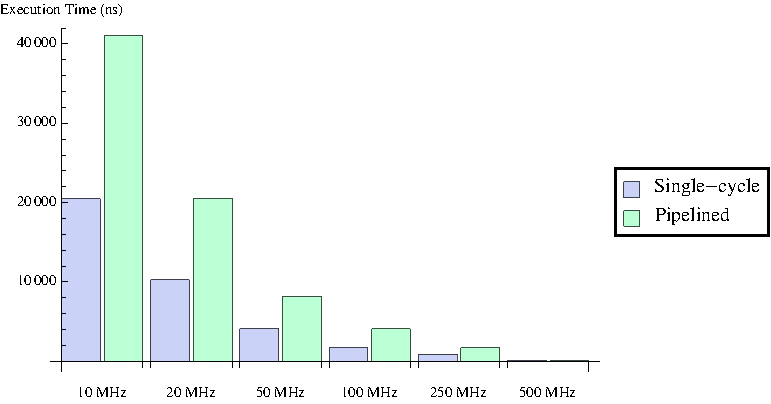
\includegraphics{fib_chart}
	\end{center}
	\caption{Fibonnaci Test}
	\label{fig:fib_chart}
\end{figure}

\begin{figure}
	\begin{center}
		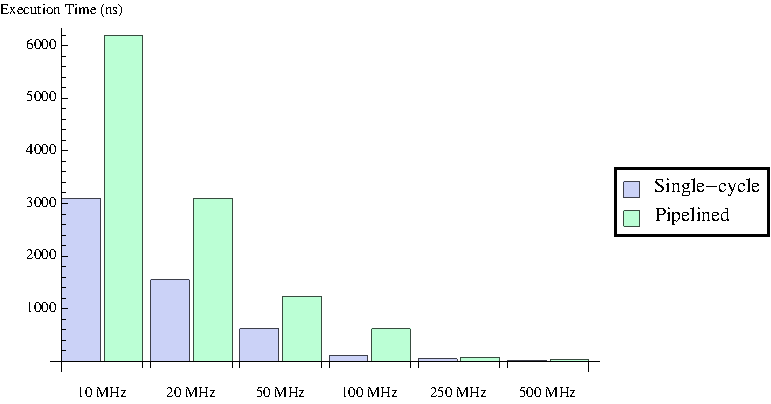
\includegraphics{mult_chart}
	\end{center}
	\caption{Multiplication Test}
	\label{fig:mult_chart}
\end{figure}

\begin{figure}
	\begin{center}
		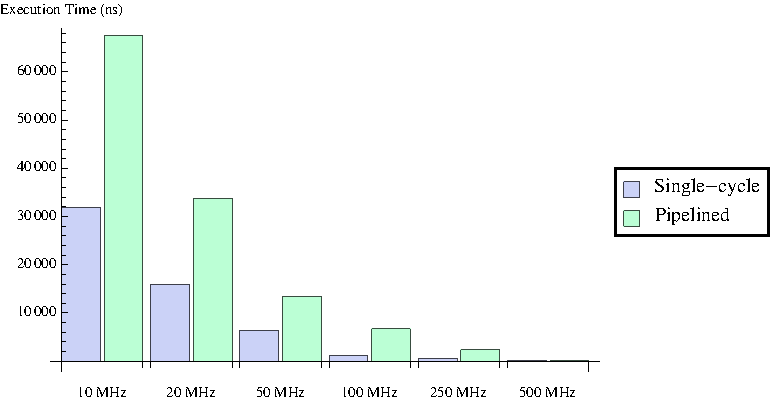
\includegraphics{search_chart}
	\end{center}
	\caption{Search Test}
	\label{fig:search_chart}
\end{figure}

  \section{Conclusion}

In this course I have designed a single-cycle and pipelined implementation of a MIPS-subset CPU. Both designs worked correctly and the pipelined design delivered a 57\% improvement in performance over the single-cycle design. The pipelined design necessarily had a higher CPI than the single-cycle design but the increase in f$_{\textrm{max}}$ more than compensated for this, improving the MIPS and latency over the simpler single-cycle design. The designs ran correctly up to clock rates slightly higher than the estimated f$_{\textrm{max}}$ returned by Quartus while exhibiting nondeterministic execution at any higher clock rates.\\

Through the course of the CPU designs, I learned first how a simple CPU is constructed, how its control logic is determined, and how a CPU design can be pipelined. The pipeline design gave me even more insight into debugging hardware designs that contain many signals and concurrent execution. By analyzing each design, I familiarized myself with how CPU performance is measured, how design choices affect performance, and how to compare the performance of designs in a meaningful manner. The single-cycle CPU has the advantage of being slightly simpler than the pipelined CPU to implement. However, the performance increase obtained by a straightforward pipelining is well worth the increase in design complexity. In terms of hardware resources used, both designs were essentially identical --- the pipelining was ``free'' in terms of resources. These CPUs could be used as an embedded processor in a System-on-a-Chip design. In this use, their performance is likely adequate as most of the heavy computations could be more quickly done in other IP-cores on the FPGA.\\

\end{document}
